\begin{figure}[h]
\center
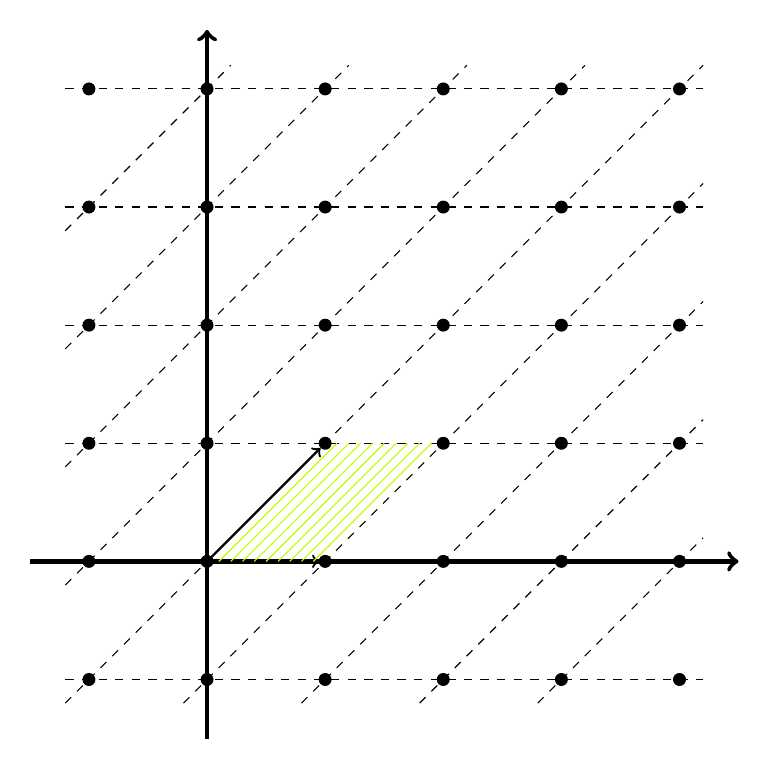
\begin{tikzpicture}[scale=1.5]

% AXES
\draw [ultra thick, ->] (-1.5, 0) -- (4.5, 0);
\draw [ultra thick, ->] (0, -1.5) -- (0, 4.5);

% BASIS VECTORS
\draw [thick, ->] (0, 0) -- (0.95, 0);
\draw [thick, ->] (0, 0) -- (0.96, 0.96);

% HORIZONTAL LINES
\draw [dashed, thin] (-1.2, 4) -- (4.2, 4);
\draw [dashed, thin] (-1.2, 3) -- (4.2, 3);
\draw [dashed, thin] (-1.2, 2) -- (4.2, 2);
\draw [dashed, thin] (-1.2, 1) -- (4.2, 1);
\draw [dashed, thin] (-1.2, -1) -- (4.2, -1);

% SKEW LINES
\draw [dashed] (-1.2, -0.2) -- (3.2, 4.2);
\draw [dashed] (-1.2, 0.8) -- (2.2, 4.2);
\draw [dashed] (-1.2, 1.8) -- (1.2, 4.2);
\draw [dashed] (-1.2, 2.8) -- (0.2, 4.2);
\draw [dashed] (-1.2, -1.2) -- (4.2, 4.2);
\draw [dashed] (-0.2, -1.2) -- (4.2, 3.2);
\draw [dashed] (0.8, -1.2) -- (4.2, 2.2);
\draw [dashed] (1.8, -1.2) -- (4.2, 1.2);
\draw [dashed] (2.8, -1.2) -- (4.2, 0.2);

% All intersection points
\draw[fill] (1,1) circle [radius=0.025];\draw[fill](-1,-1)circle [radius=0.050];\draw[fill](-1,0)circle [radius=0.050];\draw[fill](0,-1)circle [radius=0.050];\draw[fill](0,0)circle [radius=0.050];\draw[fill](1,-1)circle [radius=0.050];\draw[fill](1,0)circle [radius=0.050];\draw[fill](2,-1)circle [radius=0.050];\draw[fill](2,0)circle [radius=0.050];\draw[fill](3,-1)circle [radius=0.050];\draw[fill](3,0)circle [radius=0.050];\draw[fill](4,-1)circle [radius=0.050];\draw[fill](4,0)circle [radius=0.050];\draw[fill](-1,1)circle [radius=0.050];\draw[fill](-1,2)circle [radius=0.050];\draw[fill](0,1)circle [radius=0.050];\draw[fill](0,2)circle [radius=0.050];\draw[fill](1,1)circle [radius=0.050];\draw[fill](1,2)circle [radius=0.050];\draw[fill](2,1)circle [radius=0.050];\draw[fill](2,2)circle [radius=0.050];\draw[fill](3,1)circle [radius=0.050];\draw[fill](3,2)circle [radius=0.050];\draw[fill](4,1)circle [radius=0.050];\draw[fill](4,2)circle [radius=0.050];\draw[fill](-1,3)circle [radius=0.050];\draw[fill](-1,4)circle [radius=0.050];\draw[fill](0,3)circle [radius=0.050];\draw[fill](0,4)circle [radius=0.050];\draw[fill](1,3)circle [radius=0.050];\draw[fill](1,4)circle [radius=0.050];\draw[fill](2,3)circle [radius=0.050];\draw[fill](2,4)circle [radius=0.050];\draw[fill](3,3)circle [radius=0.050];\draw[fill](3,4)circle [radius=0.050];\draw[fill](4,3)circle [radius=0.050];\draw[fill](4,4)circle [radius=0.050];

% Fundamental paraleliped (?)

\draw[thin,color=lime] (0.1,0) -- (1.1, 1);
\draw[thin,color=lime] (0.2,0) -- (1.2, 1);
\draw[thin,color=lime] (0.3,0) -- (1.3, 1);
\draw[thin,color=lime] (0.4,0) -- (1.4, 1);
\draw[thin,color=lime] (0.5,0) -- (1.5, 1);
\draw[thin,color=lime] (0.6,0) -- (1.6, 1);
\draw[thin,color=lime] (0.7,0) -- (1.7, 1);
\draw[thin,color=lime] (0.8,0) -- (1.8, 1);
\draw[thin,color=lime] (0.9,0) -- (1.9, 1);



\end{tikzpicture}
\caption{Lattice with basis \(\mathfrak{B} = \{(1, 0), (1, 1)\}\). This lattice is isomorphic to the lattice with basis vectors \((1, 0)\) and \((-1, 1)\).}
\label{Figure:Lattice1}
\end{figure}